\documentclass[11pt, oneside]{book}

\usepackage{hyperref}
\hypersetup{
    colorlinks=true,
    linkcolor=blue,
    filecolor=magenta,      
    urlcolor=blue,
}
\usepackage{xurl}

\usepackage[inline]{enumitem}
\usepackage{pdfpages}
\usepackage{nameref}

\usepackage{xepersian}
\settextfont{Yas}
\setdigitfont{Yas}

\begin{document}
\frontmatter
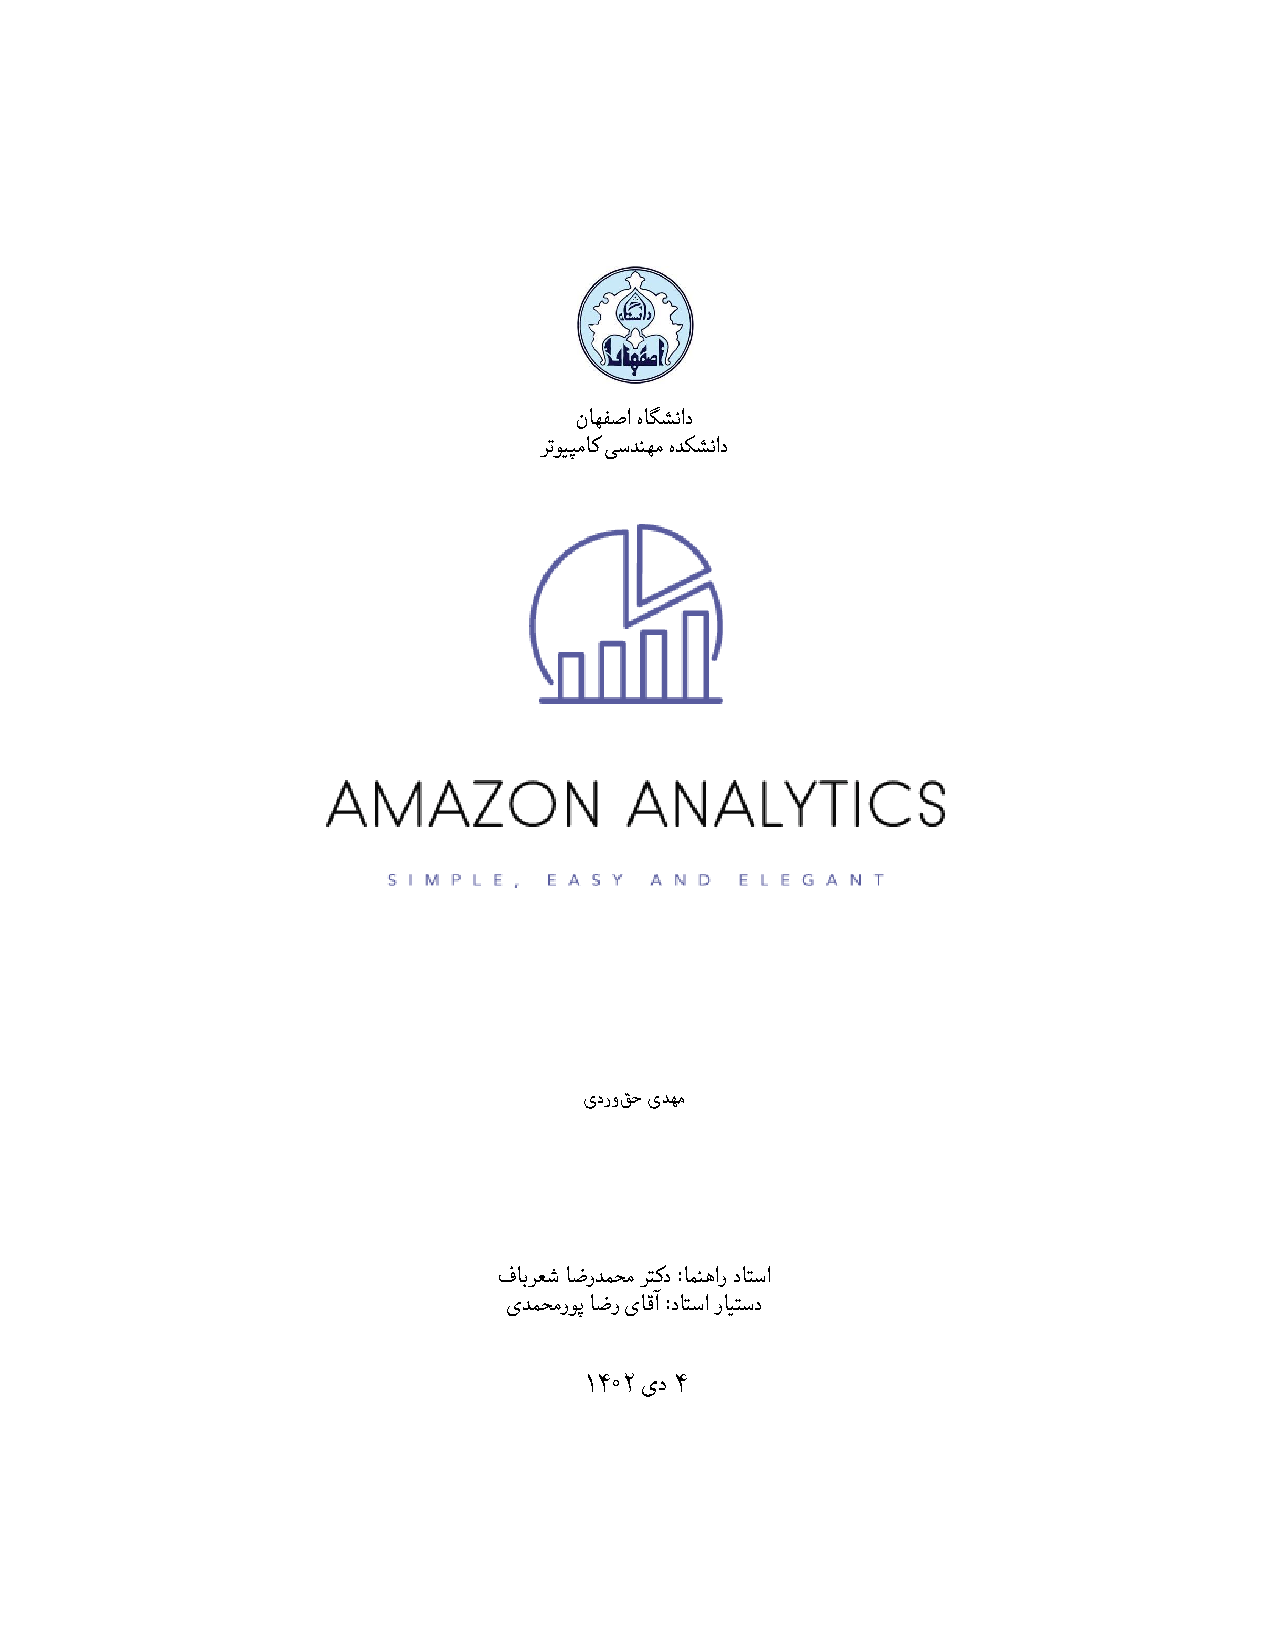
\includepdf{../titlepage/atitle}
\tableofcontents
\mainmatter

\chapter{توضیحات نسخه دمو}
در این فصل به بررسی آنچه که از پروژه‌ی 
\lr{Amazon Analytics}
به صورت دمو پیاده‌سازی می‌شود، پرداخته می‌شود. آنچه که لازم به ذکر است این‌ست که، تمامی مطالعات صورت گرفته برای پروژه‌ی
\lr{Amazon Analytics}
انجام شده، بر اساس پیاده‌سازی از صفر بوده، و همچنین با توجه به فاز سوم پروژه، نیازمند حداقل ۱۳ ماه برای پیاده‌سازی است. به همین جهت، نسخه‌ی دمو تنها قسمت کوچکی از اصل پروژه خواهد بود.

نسخه‌ی دمو قرار است یک وب اپلیکیشن باشد که ۴ قسمت اصلی دارد: 
\begin{enumerate*}
\item 
بخش کاربران،
\item 
بخش 
\lr{Stock}،
\item 
بخش 
\lr{Site}
و
\item
بخش 
\lr{Shipment}. 
\end{enumerate*}
در هر یک از این بخش‌ها، اطلاعاتی که داده‌هایش در پایگاه‌های داده‌ای در سیستم ذخیره‌ هستند، به شکل‌های 
\begin{enumerate*}
\item 
جدول و
\item 
نمودار میله‌ای
\end{enumerate*}
نشان داده می‌شوند.
\section{قسمت‌های نسخه‌ی دمو}
نسخه‌ی دمو قرار است که بر اساس یک سری داده‌ی ذخیره شده، خروجی‌های مختلفی که در پروژه به آنها پرداخته شده بود، را نشان بدهد. در این بخش قسمت‌های مختلف را نام برده و به بررسی خروجی آنها می‌پردازیم.

\subsection{بخش کاربران}\label{ssec:users}

\subsection{بخش \lr{Stock}}\label{ssec:stock}

\subsection{بخش \lr{Site}}\label{ssec:site}

\subsection{بخش \lr{Shipment}}\label{ssec:shipment}

\end{document}